% ============================================================
%  THAPAR INSTITUTE – PROJECT SEMESTER REPORT TEMPLATE
%  Compiler: pdfLaTeX (default Overleaf compiler)
% ============================================================

\documentclass[12pt, a4paper, oneside]{report}

% ── Times New Roman equivalent (pdfLaTeX compatible) ────────
\usepackage{mathptmx}
\usepackage[T1]{fontenc}
\usepackage{hyperref}
\usepackage[utf8]{inputenc}
\usepackage{pdfpages}


% ── Page geometry: 1 inch all sides ─────────────────────────
\usepackage[top=1in, bottom=1in, left=1in, right=1in]{geometry}

% ── Line spacing ─────────────────────────────────────────────
\usepackage{setspace}
\setstretch{1.5}

% ── Justification ───────────────────────────────────────────
\usepackage{microtype}
\usepackage{ragged2e}

% ── List spacing ────────────────────────────────────────────
\usepackage{enumitem}
\setlist[enumerate]{topsep=4pt, itemsep=3pt, parsep=0pt, partopsep=0pt}

% ── Heading format ──────────────────────────────────────────
\usepackage{titlesec}

\renewcommand{\thesection}{\arabic{chapter}.\arabic{section}}
\renewcommand{\thesubsection}{\thesection.\arabic{subsection}}

% Chapter = 16 pt
\titleformat{\chapter}[block]
  {\fontsize{16}{19.2}\selectfont\bfseries}
  {\thechapter.}{0.5em}{}
\titlespacing*{\chapter}{0pt}{0pt}{12pt}

% Section = 14 pt
\titleformat{\section}[block]
  {\fontsize{14}{16.8}\selectfont\bfseries}
  {\thesection}{0.5em}{}
\titlespacing*{\section}{0pt}{10pt}{4pt}

% Subsection = 12 pt
\titleformat{\subsection}[block]
  {\fontsize{12}{14.4}\selectfont\bfseries}
  {\thesubsection}{0.5em}{}
\titlespacing*{\subsection}{0pt}{8pt}{2pt}

\setcounter{secnumdepth}{3}
\setcounter{tocdepth}{3}

% ── Remove default "Chapter N" banner and top vspace ────────
\usepackage{etoolbox}
\makeatletter
\patchcmd{\@makechapterhead}{\vspace*{50\p@}}{}{}{}
\patchcmd{\@makeschapterhead}{\vspace*{50\p@}}{}{}{}
\makeatother

% ── Page numbering ───────────────────────────────────────────
\usepackage{fancyhdr}
\pagestyle{fancy}
\fancyhf{}
\fancyfoot[C]{\thepage}
\renewcommand{\headrulewidth}{0pt}
\renewcommand{\footrulewidth}{0pt}
\fancypagestyle{plain}{
  \fancyhf{}
  \fancyfoot[C]{\thepage}
  \renewcommand{\headrulewidth}{0pt}
}

% ── Figures and tables ───────────────────────────────────────
\usepackage{graphicx}
\usepackage{caption}
\captionsetup[figure]{name=Figure, labelfont=bf, labelsep=colon,
                      justification=centering, font={stretch=1.5}}
\captionsetup[table] {name=Table,  labelfont=bf, labelsep=colon,
                      justification=centering, font={stretch=1.5}}
\usepackage{booktabs}

% ── Float spacing ────────────────────────────────────────────
\setlength{\intextsep}{8pt}
\setlength{\textfloatsep}{8pt}
\setlength{\floatsep}{6pt}

% ── TOC formatting ──────────────────────────────────────────
\usepackage{tocloft}
\renewcommand{\cfttoctitlefont}{\fontsize{16}{19.2}\selectfont\bfseries}
\renewcommand{\cftloftitlefont}{\fontsize{16}{19.2}\selectfont\bfseries}
\renewcommand{\cftlottitlefont}{\fontsize{16}{19.2}\selectfont\bfseries}
\renewcommand{\cftchapleader}{\cftdotfill{\cftdotsep}}
\renewcommand{\cftchapfont}{\bfseries}
\renewcommand{\cftchappagefont}{\bfseries}

% ── Hyperref ────────────────────────────────────────────────
\usepackage{hyperref}
\hypersetup{colorlinks=true, linkcolor=black, urlcolor=black, citecolor=black,
            pdftitle={Project Semester Report}}

% ── Paragraph spacing ───────────────────────────────────────
\setlength{\parindent}{0pt}
\setlength{\parskip}{4pt}

% ============================================================
\begin{document}

% -------------------------------------------------------
% COVER PAGE
% -------------------------------------------------------
\begin{titlepage}
\thispagestyle{empty}
\begin{center}


{\fontsize{18}{22}\selectfont\bfseries PROJECT SEMESTER REPORT}

\vspace{0.6cm}

{\fontsize{18}{22}\selectfont\bfseries Frontend Observability}

\vspace{0.6cm}

{\fontsize{13}{15}\selectfont by}

\vspace{0.5cm}

{\fontsize{16}{18}\selectfont\bfseries Rachit Bansal}

\vspace{0.4cm}

{\fontsize{14}{16}\selectfont\bfseries Roll No. 102203155}

\vspace{0.8cm}

{\fontsize{13}{15}\selectfont Under the Guidance of}

\vspace{0.4cm}

{\fontsize{13}{15}\selectfont\bfseries
Faculty Mentor: Dr. Chinmaya Panigrahy
}

{\fontsize{12}{14}\selectfont
Assistant Professor, CSED, TIET, Patiala
}

\vspace{0.15cm}

{\fontsize{13}{15}\selectfont
and
}

\vspace{0.15cm}

{\fontsize{13}{15}\selectfont\bfseries
Industrial Mentor: Debangan Bhattacharyya
}

{\fontsize{12}{14}\selectfont
Software Engineer at Birla Pivot
}

\vspace{0.4cm}


\includegraphics[width=0.35\textwidth]{image.png}

\vspace{0.2cm}

{\fontsize{13}{15}\selectfont Submitted to the}

\vspace{0.2cm}

{\fontsize{14}{18}\selectfont\bfseries
Computer Science \& Engineering Department
}

{\fontsize{14}{16}\selectfont\bfseries
Thapar Institute of Engineering \& Technology, Patiala
}

\vspace{0.5cm}

{\fontsize{13}{15}\selectfont
In Partial Fulfillment of the Requirements for the Degree of
}

\vspace{0.2cm}

{\fontsize{13}{15}\selectfont\bfseries
Bachelor of Engineering in Computer Engineering
}

{\fontsize{13}{15}\selectfont\bfseries
Thapar Institute of Engineering \& Technology, Patiala
}

\vspace{0.3cm}

{\fontsize{13}{15}\selectfont\bfseries June 2026}

\end{center}
\end{titlepage}

% ============================================================
%  FRONT MATTER  —  Roman page numbers
% ============================================================
\clearpage
\pagenumbering{roman}
\setcounter{page}{1}

% ── Abstract ────────────────────────────────────────────────
\thispagestyle{plain}

\noindent{\fontsize{16}{18}\selectfont\bfseries Frontend Observability}

\vspace{0.15in}

\noindent{\fontsize{12}{14}\selectfont by {{Rachit Bansal}}}

\vspace{0.1in}

\noindent{\fontsize{12}{14}\selectfont Place of Work: Birla Pivot}

\vspace{0.15in}

\noindent{\fontsize{12}{14}\selectfont
Submitted to the Computer Science \& Engineering Department, Thapar Institute of Engineering \& Technology, Patiala}

\vspace{0.15in}

\noindent{\fontsize{12}{14}\selectfont June 2026}

\vspace{0.15in}

\noindent{\fontsize{12}{14}\selectfont
In Partial Fulfillment of the Requirements for the Degree of Bachelor of Engineering in Computer Engineering}

\vspace{0.15in}

\noindent{\fontsize{14}{16}\selectfont\bfseries Abstract:}

\vspace{0.05in}

{\fontsize{12}{14}\selectfont
Modern web applications require continuous monitoring to ensure reliability, performance, and a seamless user experience. This project focused on designing and implementing a Frontend Observability solution to provide real-time visibility into application health, user interactions, frontend errors, and API behavior.

A custom observability framework was developed and integrated into the existing infrastructure to address organization-specific monitoring requirements that were not adequately supported by available off-the-shelf solutions. The system captures frontend exceptions, network failures, performance metrics, user activity events, and application health indicators, enabling comprehensive monitoring of client-side application behavior.

The collected telemetry data is processed through a scalable monitoring pipeline and visualized using dashboards and centralized logging solutions such as Grafana and Kibana. Real-time alerting mechanisms were also implemented to proactively detect critical issues and reduce troubleshooting time.

A key contribution of this project is the development of custom observability workflows and instrumentation strategies tailored to the organization's architecture, deployment model, and operational processes.

The implemented solution improves operational visibility, accelerates issue resolution, and enables data-driven decision-making, ultimately contributing to enhanced application reliability, performance, and user satisfaction.
}

\vspace{0.3in}

\noindent
Author
\hspace{1.5cm}
\underline{\hspace{8cm}}

\vspace{-0.30cm}

\hspace*{2.8cm}
(Rachit Bansal)

\vspace{0.4in}

\noindent
Certified by
\hspace{0.8cm}
\underline{\hspace{8cm}}

\vspace{-0.30cm}

\hspace*{2.8cm}
(Industrial Coordinator / Mentor)

\vspace{0.4in}

\noindent
Certified by
\hspace{0.8cm}
\underline{\hspace{8cm}}

\vspace{-0.30cm}

\hspace*{2.8cm}
(Faculty Mentor)

\newpage

% ── Industrial Mentor Signature Email ─────────────────────────────────
\begin{center}
    {\fontsize{16}{19.2}\selectfont\bfseries
    Industrial Mentor Signature Email}
\end{center}

\begin{center}
    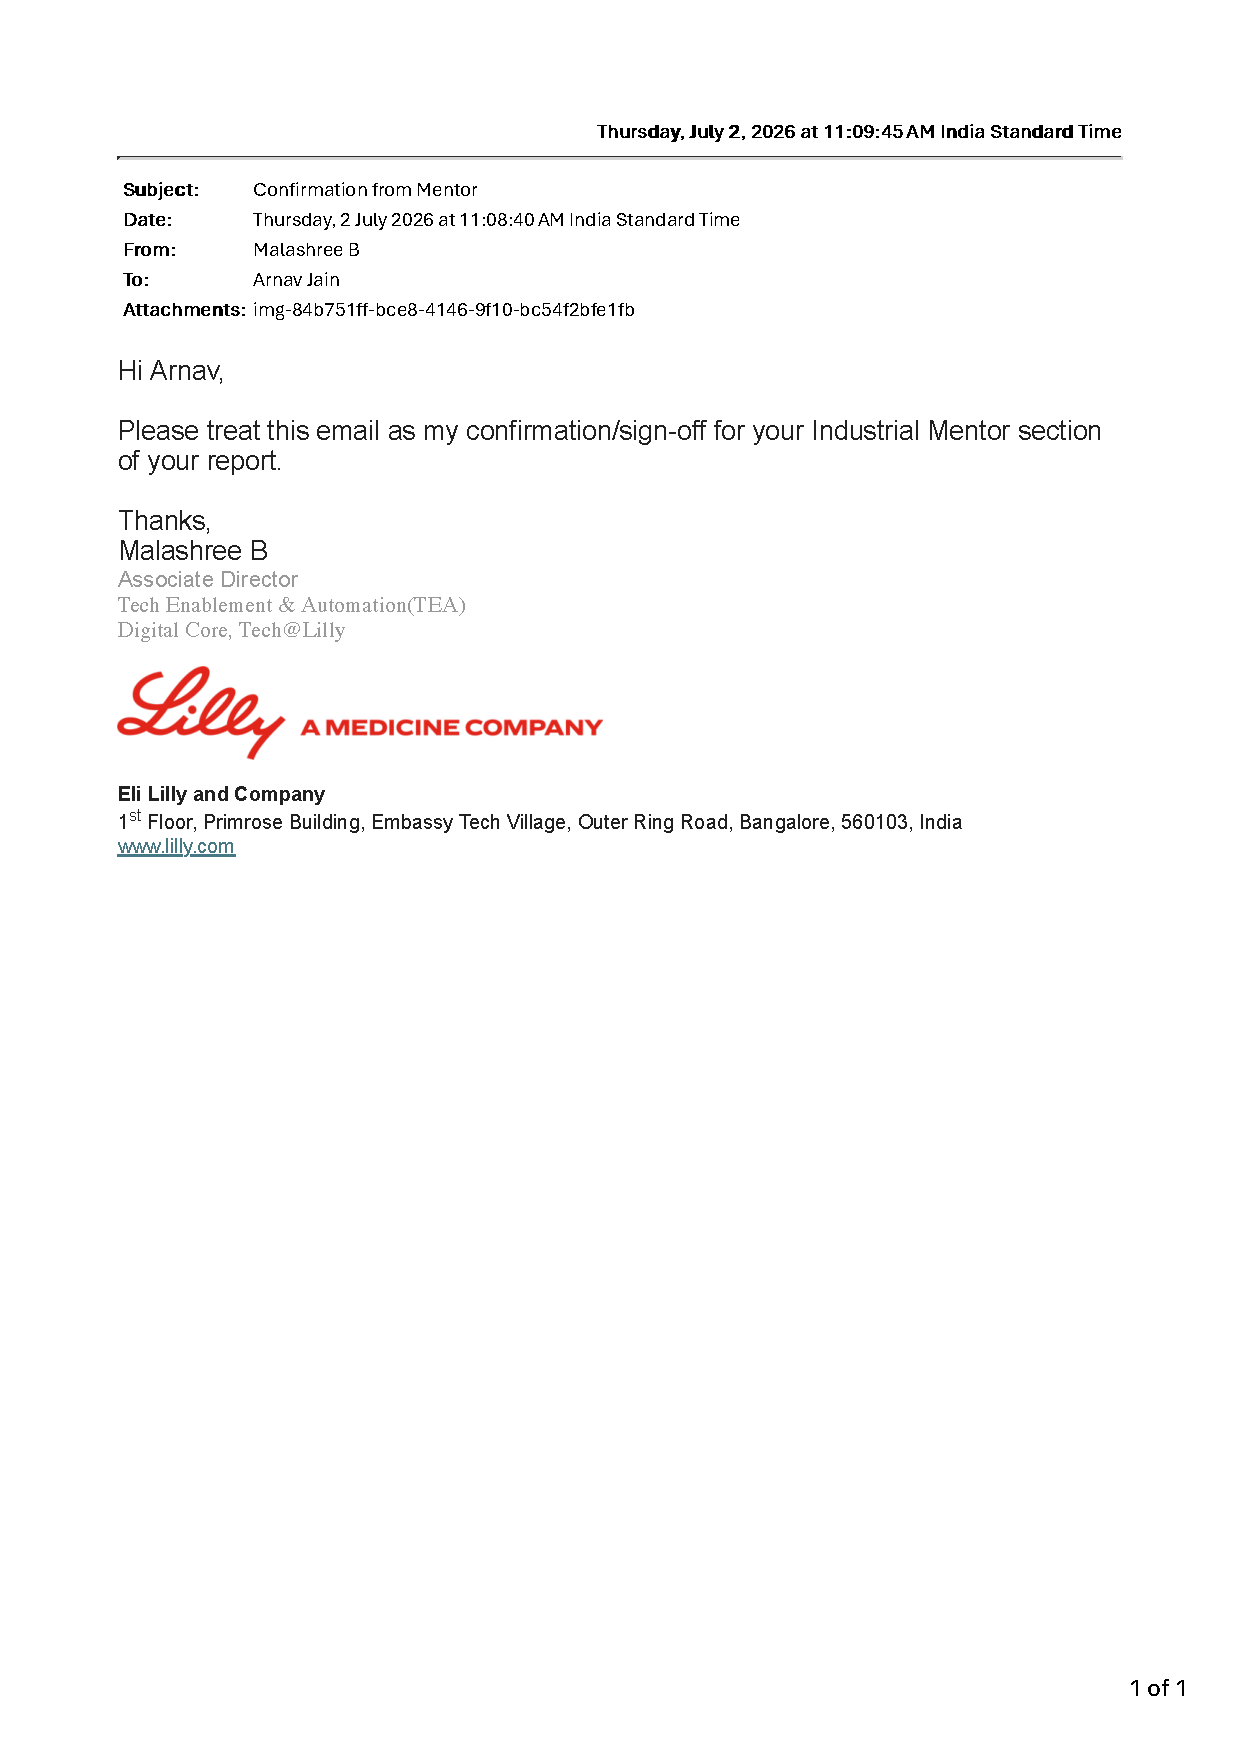
\includegraphics[height=0.9\textheight,keepaspectratio]{IndustrialMentorSign.pdf}
\end{center}

\newpage

% ── Company Certificate ─────────────────────────────────────
\thispagestyle{plain}
\begin{center}
  {\fontsize{16}{19.2}\selectfont\bfseries
    CERTIFICATE (PROJECT SEMESTER TRAINING)\\[6pt]
    FROM THE COMPANY OR ORGANIZATION}
\end{center}

% \vspace{0.3in}

% \noindent Candidate must place the scanned or original copy of the certificate
% related to completion of the project semester as received from the software
% company / research institute.

% \includepdf[pages=1]{Project_Sem_Certificate.pdf}
\begin{center}
    \includegraphics[height=0.90\textheight,keepaspectratio]{Project_Sem_Certificate.pdf}
\end{center}

\newpage

% ── Table of Contents ───────────────────────────────────────
\tableofcontents
\newpage

% ── List of Figures ─────────────────────────────────────────
\listoffigures
\addcontentsline{toc}{chapter}{List of Figures}
\newpage

% ── List of Tables ──────────────────────────────────────────
\listoftables
\addcontentsline{toc}{chapter}{List of Tables}
\newpage

% ============================================================
%  MAIN MATTER  —  Arabic page numbers, restart from 1
% ============================================================
\pagenumbering{arabic}
\setcounter{page}{1}

% ============================================================
%  1.  COMPANY PROFILE
% ============================================================
\chapter{Company Profile}

\section{Overview of the Company}

Birla Pivot is the B2B e-commerce platform of the Aditya Birla Group, one of India's leading multinational conglomerates with a strong presence across manufacturing, financial services, retail, telecommunications, metals, cement, chemicals, and other industries. Birla Pivot aims to digitally transform the procurement and supply chain ecosystem by providing businesses with a unified platform for sourcing industrial products and services. The organization focuses on leveraging technology to improve efficiency, transparency, and accessibility within the B2B commerce sector.

\section{Products and Services}

Birla Pivot offers a comprehensive digital marketplace that connects buyers and sellers across multiple industrial categories. The platform provides businesses with access to a wide range of products, including industrial equipment, construction materials, electrical supplies, safety products, and other enterprise procurement requirements. In addition to product discovery and purchasing, the platform supports digital transactions, supplier management, order tracking, and streamlined procurement workflows to enhance operational efficiency.

\section{Technology and Innovation}

Technology plays a central role in Birla Pivot's vision of creating a modern and scalable B2B commerce ecosystem. The organization adopts cloud-based infrastructure, data-driven decision-making, modern web technologies, observability solutions, and automation practices to build reliable and high-performing digital platforms. Continuous innovation is encouraged through the development of scalable systems, monitoring frameworks, analytics solutions, and customer-centric digital experiences.

\section{Internship Experience and Learning Environment}

My internship at Birla Pivot provided valuable exposure to large-scale enterprise application development and modern software engineering practices. I worked closely with experienced professionals and contributed to the design and implementation of a Frontend Observability solution aimed at improving application monitoring, reliability, and operational visibility. The collaborative work environment encouraged learning, problem-solving, ownership, and innovation, enabling me to gain practical experience in frontend engineering, monitoring systems, logging, dashboarding, and production-grade software development practices.

\vspace{0.5cm}
\begin{figure}[h]
    \centering
    \includegraphics[width=0.40\textwidth]{Birla_Pivot.png}
    \caption{Birla Pivot Logo}
    \label{fig:Birla_Pivot}
\end{figure}

% ============================================================
%  2.  INTRODUCTION
% ============================================================
\chapter{Introduction}

As modern web applications continue to grow in scale and complexity, ensuring a seamless user experience has become increasingly challenging. While backend systems are typically equipped with robust monitoring solutions, understanding what users actually experience on the frontend remains a difficult problem. A failed API call, a JavaScript exception, a slow page load, or a broken user journey can directly impact business operations, yet these issues often go unnoticed until reported by end users.

During my internship at Birla Pivot, I worked on building a Frontend Observability platform aimed at bridging this visibility gap. The goal of the project was to provide engineering teams with real-time insights into application behavior, user interactions, frontend errors, API performance, and overall application health from the user's perspective.

One of the key challenges was that the existing monitoring ecosystem was primarily focused on infrastructure and backend services. Off-the-shelf frontend monitoring solutions did not align completely with the organization's architecture, workflows, and operational requirements. To address this, a custom observability framework was designed and implemented from the ground up, enabling seamless integration with the existing technology stack and monitoring infrastructure.

The solution involved frontend instrumentation, centralized event collection, custom logging pipelines, dashboard creation, real-time alerting, and operational analytics. Technologies such as JavaScript/TypeScript, React, Grafana, Kibana, Elasticsearch, and cloud-native monitoring components were leveraged to build a scalable and production-ready system.

The implemented platform provides end-to-end visibility into frontend application health, accelerates issue detection and troubleshooting, supports data-driven decision making, and establishes a strong foundation for future observability initiatives within the organization. Beyond the technical implementation, the project offered valuable exposure to large-scale software systems, monitoring architectures, production operations, and modern engineering practices used in enterprise environments.

% ============================================================
%  3.  BACKGROUND
% ============================================================
\chapter{Background}

\section{Frontend Observability in Modern Web Applications}

Modern web applications have evolved into highly distributed systems involving multiple frontend modules, backend services, third-party integrations, and complex user workflows. While organizations commonly invest in backend and infrastructure monitoring, obtaining visibility into the actual experience of end users remains a significant challenge.

Issues such as JavaScript exceptions, failed API requests, slow page loads, browser-specific problems, and network connectivity failures directly affect users and business operations. However, these issues are often difficult to detect through traditional monitoring solutions because they originate within the user's browser environment. This creates a visibility gap between system health and user experience, making frontend observability an increasingly important aspect of modern software engineering.

\section{Existing Monitoring Landscape}

At Birla Pivot, monitoring capabilities were primarily focused on infrastructure components, backend services, and operational metrics. While these systems provided valuable insights into server-side behavior, they offered limited visibility into frontend-specific incidents and user-facing issues.

As a result, diagnosing frontend failures often required manual investigation across multiple systems and teams. Understanding whether an issue originated from the frontend application, a network failure, a backend service, or an external dependency was frequently a time-consuming process. The absence of centralized frontend visibility highlighted the need for a dedicated observability solution capable of providing actionable insights into application behavior from the user's perspective.

\section{Proof of Concept and Technology Evaluation}

Before introducing any changes into production systems, a dedicated Proof of Concept (PoC) was developed in a separate project environment. Given the scale and potential impact of the proposed frontend observability solution, direct implementation within the organization's applications was considered inappropriate during the initial stages. The PoC provided a controlled environment for experimentation, validation, and stakeholder alignment before proceeding with production adoption.

The primary objective of the PoC was to evaluate different approaches for frontend telemetry collection, centralized logging, monitoring, and visualization. During this phase, multiple technologies and architectural patterns were explored, including centralized logging solutions such as Loki and other observability components. The evaluation focused on understanding integration requirements, scalability characteristics, operational feasibility, and the suitability of different technologies for frontend monitoring use cases.

In addition to evaluating open-source observability components, commercially available frontend monitoring platforms were also studied to understand their capabilities, integration requirements, and operational implications. While these solutions offered several advanced features, their adoption would have introduced additional licensing, onboarding, and long-term operational costs.

During the evaluation phase, Loki-based logging architectures were also explored as part of the Proof of Concept. Although technically feasible, introducing a dedicated logging stack would have required additional infrastructure management and operational overhead. Since a mature OpenSearch-based ecosystem already existed within the organization, it was determined that leveraging the existing infrastructure would provide better integration, operational simplicity, and long-term maintainability.

The evaluation ultimately led to the selection of a custom observability architecture that maximized reuse of existing organizational capabilities while minimizing additional dependencies and operational costs.

The PoC also helped identify potential implementation challenges and provided valuable insights into how telemetry data could be collected, processed, stored, and visualized effectively. The findings from these experiments established a clearer understanding of project requirements and enabled informed technology selection for the final solution.

In addition to technical validation, the PoC served as an important communication tool between frontend engineers, platform teams, and management. By demonstrating practical use cases and expected outcomes, it enabled stakeholders to visualize the proposed solution, provide early feedback, and align on project goals, implementation feasibility, and future requirements before production deployment.

\section{Observability Solution Evaluation}

As part of the technology evaluation process, different observability approaches were compared based on functional capabilities, operational requirements, and long-term sustainability.

\begin{table}[h]
\centering
\caption{Comparison of Observability Approaches}
\label{tab:observability-comparison}
\begin{tabular}{|p{6cm}|p{5cm}|p{5cm}|}
\hline
\textbf{Criteria} & \textbf{Commercial Observability Platforms} & \textbf{Proposed Solution} \\
\hline

Frontend Error Monitoring &
Supported &
Supported
\\
\hline

API Performance Monitoring &
Supported &
Supported
\\
\hline

Dashboarding and Visualization &
Supported &
Supported
\\
\hline

Vendor Lock-in &
High &
None
\\
\hline

Customization Flexibility &
Limited by Vendor &
High
\\
\hline

Integration with Existing Infrastructure &
Moderate &
High
\\
\hline

Licensing Requirements &
Required &
Not Required
\\
\hline

Additional Infrastructure Onboarding &
Required &
Minimal
\\
\hline

Long-Term Operational Cost &
Higher &
Lower
\\
\hline

\end{tabular}
\end{table}

The evaluation demonstrated that a custom-built solution could provide the required observability capabilities while offering greater flexibility, reduced operational complexity, and significant long-term cost advantages. These findings supported the decision to proceed with the proposed architecture for the implementation phase.

\section{Evolution of Project Requirements}

The project initially began with the objective of improving visibility into frontend errors and API failures. However, as discussions progressed with different stakeholders, the scope expanded significantly.

Additional requirements emerged around application performance monitoring, user session visibility, browser and device analytics, network failure tracking, operational dashboards, and proactive issue detection. The project gradually evolved from a simple monitoring initiative into a broader frontend observability platform capable of supporting operational, debugging, and analytical use cases.

This iterative requirement gathering process played a crucial role in shaping the final vision of the project and ensured that the solution addressed the needs of multiple teams across the organization.

\begin{figure}[h]
    \centering
    \includegraphics[width=0.7\textwidth]{Broad_Workflow.png}
    \caption{Overall Workflow}
    \label{fig:Broad_Workflow}
\end{figure}

This workflow, illustrated in Figure \ref{fig:Broad_Workflow}, represents the overall workflow of the frontend observability.

\section{Motivation for the Project}

The motivation behind this project extended far beyond implementing a new monitoring tool. It presented an opportunity to work on a completely different engineering domain involving observability, telemetry collection, monitoring systems, and operational analytics.

Unlike traditional feature development, the project required understanding multiple technologies, evaluating different architectural approaches, and designing a solution that could be adopted across teams. Since the frontend acts as the primary interaction layer between users and business services, issues occurring at this layer can directly impact user experience, business workflows, API consumption, and overall platform reliability.

The potential organizational impact of the project served as a strong source of motivation. Successfully implementing a frontend observability framework would not only improve issue detection and troubleshooting but also establish a long-term foundation for monitoring and operational excellence across the organization. The combination of technical complexity, cross-functional collaboration, and company-wide relevance made this project both challenging and highly rewarding.

% ============================================================
%  4.  OBJECTIVES
% ============================================================
\chapter{Objectives}

The primary objective of this project was to design and implement a comprehensive Frontend Observability platform capable of providing real-time visibility into application behavior, performance, and reliability. To achieve this goal, the following objectives were defined:

\begin{enumerate}

\item \textbf{Evaluation of Frontend Observability Approaches.}
To study and evaluate different frontend observability approaches and technologies through a dedicated Proof of Concept (PoC), and identify an architecture suitable for the organization's requirements.

\item \textbf{Development of a Telemetry Collection Framework.}
To design and implement a scalable, vendor-independent telemetry collection framework capable of capturing frontend events, API interactions, application errors, and performance metrics from user browsers.

\item \textbf{Establishment of an End-to-End Observability Pipeline.}
To establish an end-to-end observability pipeline for collecting, processing, transforming, and storing frontend telemetry data using modern observability standards and tools.

\item \textbf{Implementation of Comprehensive Monitoring Capabilities.}
To implement comprehensive monitoring capabilities including frontend error tracking, API performance monitoring, network failure detection, Core Web Vitals measurement, user session analytics, and browser-level insights.

\item \textbf{Development of Dashboards and Visualization Solutions.}
To develop centralized dashboards, log analytics, and visualization solutions that provide engineering teams with actionable insights into application health, user experience, and operational performance.

\item \textbf{Enabling Proactive Issue Detection and Troubleshooting.}
To enable proactive issue detection and faster troubleshooting through real-time monitoring, structured telemetry, centralized logging, and alerting mechanisms integrated with the existing organizational infrastructure.

\end{enumerate}

% ============================================================
%  5.  METHODOLOGY
% ============================================================
\chapter{Methodology}

This chapter describes the approach followed to achieve the objectives of the project. The implementation was carried out in multiple phases, beginning with requirement analysis and technology evaluation, followed by architecture design, telemetry collection, data processing, visualization, and operational monitoring.

\section{Requirement Analysis and Planning}

The project commenced with discussions involving frontend engineers, platform teams, and management to identify existing monitoring gaps and operational challenges. Multiple use cases were studied, including frontend error tracking, API performance monitoring, user session visibility, performance measurement, and proactive issue detection.

Based on the identified requirements, a roadmap was prepared to design a frontend observability platform capable of providing end-to-end visibility into application behavior while integrating seamlessly with the existing organizational infrastructure.

\section{Proof of Concept Development}

Before introducing any changes into production systems, a dedicated Proof of Concept (PoC) was developed using a separate local project environment.

The PoC focused on the following objectives:

\begin{itemize}
    \item Evaluating frontend instrumentation approaches.
    \item Understanding telemetry collection mechanisms.
    \item Studying centralized logging architectures.
    \item Validating data storage strategies.
    \item Comparing visualization and monitoring solutions.
    \item Assessing scalability and operational feasibility.
\end{itemize}

Multiple observability technologies and architectural approaches were explored during this phase, helping establish the technical foundation for the final implementation and providing confidence before proceeding towards a production-ready solution.

\begin{figure}[h]
  \centering
  \includegraphics[width=1.0\textwidth]{POC.png}
  \caption{Proof of Concept Evaluation Workflow}
  \label{fig:POC}
\end{figure}

\section{Final Architecture Design}

Based on the insights gained during the Proof of Concept (PoC) phase, a custom frontend observability architecture was designed. The architecture follows a telemetry-driven approach in which frontend events are collected, processed, transformed, stored, and visualized through a centralized observability pipeline.

The major components of the architecture and their responsibilities are summarized in Table~\ref{tab:architecture-components}.
\n
\begin{table}[h]
\centering
\caption{Major Components of the Observability Platform}
\label{tab:architecture-components}
\begin{tabular}{|p{6cm}|p{10cm}|}
\hline
\textbf{Component} & \textbf{Responsibility} \\
\hline

Faro SDK &
Frontend instrumentation and telemetry generation. Captures user interactions, errors, performance metrics, and application events from the frontend application.
\\
\hline

Grafana Alloy &
Collects telemetry data from multiple sources and forwards it to downstream observability components for further processing and storage.
\\
\hline

OpenTelemetry &
Provides a standardized framework for generating, collecting, and transporting telemetry data across the observability ecosystem.
\\
\hline

Logstash &
Processes, transforms, enriches, and formats telemetry data before forwarding it to the storage layer.
\\
\hline

OpenSearch &
Serves as the centralized storage and indexing engine for logs and telemetry data, enabling efficient querying and analysis.
\\
\hline

Grafana &
Provides dashboards, visualizations, and monitoring interfaces for analyzing frontend performance, errors, and user behavior.
\\
\hline

Alerting Layer &
Generates proactive notifications and alerts based on predefined thresholds, anomalies, or critical application events.
\\
\hline

\end{tabular}
\end{table}

\newpage

Regular check-ins with the mentor ensured alignment with organizational expectations and technical standards. The mentor provided requirement specifications, reviewed implementation decisions at key milestones, and offered guidance whenever design or technical challenges were encountered. This structure encouraged independent problem-solving while maintaining appropriate oversight and direction throughout the project lifecycle.

\subsection{End-to-End Data Flow}

\begin{figure}[h]
  \centering
  \includegraphics[width=0.5\textwidth]{obsFlow.png}
  \caption{observability pipeline flow}
  \label{fig:obsFlow}
\end{figure}

The architecture was designed to be scalable, vendor-independent, and extensible for future observability requirements.

\newpage

\section{Architectural Decisions and Customizations}

While several observability tools provide out-of-the-box monitoring capabilities, the requirements of the project extended beyond the functionality offered by default implementations. As a result, multiple architectural customizations were introduced to align the solution with organizational requirements and existing infrastructure.

One of the key design decisions involved leveraging the organization's existing OpenSearch ecosystem instead of introducing a separate logging infrastructure. This reduced deployment complexity, avoided additional operational ownership, and enabled seamless integration with existing monitoring workflows.

Several custom telemetry collection mechanisms were also implemented to improve observability coverage. These included enhanced API instrumentation, custom event classification, structured error categorization, network failure detection, environment-aware monitoring, and telemetry enrichment for improved analytics and debugging capabilities.

These customizations enabled the platform to address organization-specific monitoring requirements while maintaining scalability, flexibility, and operational efficiency.

\section{Frontend Instrumentation}

Frontend instrumentation was implemented using the Grafana Faro SDK. The instrumentation layer was responsible for capturing various types of telemetry data generated by the frontend application.

The instrumentation focused on collecting the following information:

\begin{itemize}
    \item JavaScript runtime exceptions.
    \item API requests and responses.
    \item Network failures.
    \item Browser information.
    \item User session metadata.
    \item Page navigation events.
    \item Core Web Vitals.
\end{itemize}

Special attention was given to ensuring minimal performance overhead while maintaining comprehensive visibility into frontend application behavior. The instrumentation was designed to operate efficiently without negatively impacting the end-user experience.

To achieve complete API visibility, instrumentation was implemented for both Fetch API and XMLHttpRequest (XHR)-based requests, ensuring monitoring coverage across all application components and communication pathways.

\section{Telemetry Collection and Processing}

Once generated within the browser, telemetry data is forwarded through a centralized processing pipeline for collection, transformation, storage, and analysis.

Grafana Alloy acts as the telemetry collection layer and forwards the collected data using OpenTelemetry standards. Logstash performs data transformation, enrichment, filtering, and routing before storing the processed records within OpenSearch. This processing pipeline ensures that telemetry data remains structured, searchable, and suitable for visualization and monitoring purposes.

The use of OpenTelemetry as the telemetry backbone provides a standardized and future-proof mechanism for collecting, transporting, and processing observability data across different components of the platform.

The primary categories of telemetry data collected during the project are summarized in Table~\ref{tab:telemetry-classification}.

\begin{table}[h]
\centering
\caption{Telemetry Data Classification}
\label{tab:telemetry-classification}
\begin{tabular}{|p{6cm}|p{10cm}|}
\hline
\textbf{Data Type} & \textbf{Purpose} \\
\hline

Event &
Used for analytics, user activity tracking, and application monitoring.
\\
\hline

Exception &
Used for identifying, diagnosing, and debugging application errors and failures.
\\
\hline

Measurement &
Used for collecting performance metrics and monitoring application health indicators.
\\
\hline

Log &
Used for capturing console messages, application logs, and operational information.
\\
\hline

\end{tabular}
\end{table}

\newpage

\section{Monitoring Implementation}

The observability platform was designed to provide comprehensive visibility across multiple operational dimensions of the frontend application. Different monitoring capabilities were implemented to ensure effective tracking of application health, performance, reliability, and user experience.

\subsection{Error Monitoring}

The error monitoring framework was implemented to capture and analyze application failures and unexpected behaviors. The system collects the following error-related telemetry:

\begin{itemize}
    \item JavaScript exceptions.
    \item HTTP 4xx errors.
    \item HTTP 5xx errors.
    \item Network failures.
    \item Console errors.
\end{itemize}

These insights enable faster root cause analysis and support proactive identification of application issues before they significantly impact users.

\subsection{API Monitoring}

API monitoring capabilities were implemented to provide visibility into backend communication and service performance. The system tracks:

\begin{itemize}
    \item API latency.
    \item Request volume.
    \item Success and failure rates.
    \item Slow APIs.
    \item Endpoint-level analytics.
\end{itemize}

This information helps identify performance bottlenecks, unstable endpoints, and service degradation trends.

\subsection{Performance Monitoring}

Frontend performance monitoring was implemented using Core Web Vitals and browser performance indicators. The following metrics are continuously monitored:

\begin{itemize}
    \item Largest Contentful Paint (LCP).
    \item First Contentful Paint (FCP).
    \item Time to First Byte (TTFB).
    \item Cumulative Layout Shift (CLS).
    \item Interaction to Next Paint (INP).
\end{itemize}

These metrics provide insights into application responsiveness, rendering efficiency, and overall user experience.

\subsection{User Session Analytics}

Session-level telemetry is collected to understand user behavior and application usage patterns. The collected insights include:

\begin{itemize}
    \item User behavior patterns.
    \item Browser distribution.
    \item Device information.
    \item Navigation trends.
\end{itemize}

These analytics support data-driven decision-making and help identify opportunities for improving usability, performance, and user engagement.

\section{Visualization and Dashboard Development}

To enable effective operational monitoring and troubleshooting, centralized dashboards were developed using Grafana. These dashboards provide real-time visibility into frontend application behavior, system performance, user activity, and operational health.

The dashboards were designed to present the following insights:

\begin{itemize}
    \item Application health overview.
    \item API performance analytics.
    \item Error trends and distribution.
    \item User session statistics.
    \item Browser and operating system insights.
    \item Performance metrics visualization.
\end{itemize}

The dashboard design was structured to support both high-level operational monitoring and detailed root-cause analysis. High-level dashboards provide a consolidated view of system health and key performance indicators, while detailed dashboards enable engineers to investigate specific issues, analyze trends, and identify potential bottlenecks within the application.

The centralized visualization layer significantly improves observability by transforming raw telemetry data into actionable insights, enabling faster troubleshooting, improved decision-making, and proactive system monitoring.

\section{Alerting and Operational Monitoring}

Real-time alerting mechanisms were implemented as part of the observability platform to proactively identify critical incidents and operational anomalies. The alerting framework continuously monitors telemetry data and generates notifications whenever predefined thresholds or conditions are violated.

Alerting rules were configured for the following scenarios:

\begin{itemize}
    \item Increased frontend error rates.
    \item API latency threshold breaches.
    \item Excessive failed requests.
    \item Application health degradation.
\end{itemize}

These alerts provide early visibility into potential issues, allowing engineering teams to respond quickly before they significantly impact end users. By automating incident detection, the platform reduces the time required for investigation, troubleshooting, and resolution.

The integration of alerting with the centralized monitoring system ensures continuous operational awareness and supports a proactive approach to maintaining application reliability, performance, and user experience.

\section{Deployment and Validation}

Following the implementation of the observability platform, the completed framework was integrated with the target frontend application and deployed across the required environments. Comprehensive validation activities were conducted to ensure the reliability, accuracy, and effectiveness of the overall solution.

The validation process focused on verifying the following aspects:

\begin{itemize}
    \item Accuracy of telemetry collection.
    \item Correctness of dashboard metrics.
    \item Reliability of data pipelines.
    \item Alert generation behavior.
    \item End-to-end observability coverage.
\end{itemize}

Testing was performed across multiple scenarios to confirm that telemetry data was correctly captured, processed, stored, and visualized throughout the observability pipeline. Additional validation ensured that alerting mechanisms were triggered appropriately when predefined conditions and thresholds were met.

Successful validation confirmed that the platform was capable of providing comprehensive visibility into frontend application behavior while maintaining reliable telemetry processing and monitoring capabilities.

% ============================================================
%  6.  OBSERVATIONS AND FINDINGS
% ============================================================
\chapter{Observations and Findings}

The implemented frontend observability platform successfully provided real-time visibility into application behavior, performance, and operational health. The collected telemetry data enabled centralized monitoring and analysis of frontend activities across different environments.

The developed dashboards provided actionable insights into frontend errors, API performance, user sessions, browser distribution, and Core Web Vitals. These visualizations simplified troubleshooting activities and improved the ability to identify issues affecting application reliability and user experience.

\section{Key Observations}

The implementation and validation phases resulted in several important observations regarding the effectiveness of the observability platform:

\begin{itemize}
    \item Frontend errors and exceptions could be tracked centrally without relying on manual user reports.
    \item API performance metrics enabled identification of slow or failing endpoints.
    \item Session analytics provided better visibility into user activity and browser usage patterns.
    \item Core Web Vitals monitoring helped evaluate frontend performance from the end-user perspective.
    \item Centralized logs improved debugging and root-cause analysis capabilities.
    \item Real-time dashboards enabled faster issue detection and operational monitoring.
\end{itemize}

\section{Key Findings}

Based on the implementation, testing, and operational observations, the following key findings were identified:

\begin{itemize}
    \item A dedicated frontend observability framework significantly improves visibility into client-side application behavior.
    \item Combining telemetry collection, centralized storage, and dashboarding creates a unified monitoring experience.
    \item Structured observability data reduces troubleshooting effort and accelerates issue resolution.
    \item The implemented architecture provides a scalable foundation for future monitoring and analytics requirements.
\end{itemize}

\section{Operational and Cost Benefits}

A significant outcome of the project was the ability to deliver enterprise-grade frontend observability while leveraging existing organizational infrastructure.

By integrating with the existing OpenSearch ecosystem and adopting open-source observability technologies, the solution avoided the need for onboarding additional commercial monitoring platforms. This eliminated recurring licensing costs, reduced procurement overhead, and avoided the operational effort associated with managing separate observability infrastructures.

The resulting architecture provides a cost-effective and scalable monitoring solution while retaining full control over telemetry data, customization capabilities, and future expansion opportunities.

\begin{figure}[h]
  \centering
  \includegraphics[width=1.0\textwidth]{grafana1.png}
  \caption{Grafana Dashboard}
  \label{fig:grafana1}
\end{figure}

\begin{figure}[h]
  \centering
  \includegraphics[width=1.0\textwidth]{grafana2.png}
  \caption{Grafana Dashboard}
  \label{fig:grafana2}
\end{figure}

\begin{figure}[h]
  \centering
  \includegraphics[width=1.0\textwidth]{kibana.png}
  \caption{Opensearch Dashboard - Logs}
  \label{fig:kibana}
\end{figure}

\newpage
% ============================================================
%  7.  CHALLENGES AND LEARNINGS
% ============================================================

% ============================================================
%  8.  LIMITATIONS
% ============================================================
\chapter{Limitations}

While the implemented frontend observability platform provides comprehensive visibility into web application behavior, certain limitations remain within the scope of the current implementation.

The solution has been designed and validated primarily for web-based frontend applications. Extending the same observability framework to mobile applications would require additional research, platform-specific instrumentation, and integration with mobile telemetry collection mechanisms.

Although the platform captures session-level analytics, application events, errors, and performance metrics, it does not provide complete user journey replay or detailed click-by-click traceability for individual users. Advanced capabilities such as session replay, interaction heatmaps, and detailed user navigation reconstruction were intentionally kept outside the scope of the project.

The observability data available within the platform is limited to the telemetry explicitly instrumented within the application. Additional business-specific events, custom analytics requirements, and domain-specific monitoring needs would require further instrumentation, configuration, and validation efforts.

Furthermore, the effectiveness of monitoring and alerting depends on the quality and completeness of the instrumentation implemented within the application. Any uninstrumented components or events may reduce overall observability coverage.

Despite these limitations, the implemented solution successfully achieves the primary objective of providing centralized frontend monitoring, operational visibility, and proactive issue detection for web applications. The platform establishes a strong foundation for future enhancements and expansion of observability capabilities.

\chapter{Conclusion and Future Work}

\section{Conclusion}

The project successfully achieved its objective of designing and implementing a comprehensive frontend observability platform for Birla Pivot. Through a structured approach involving requirement analysis, proof-of-concept development, architecture evaluation, and production implementation, a scalable and vendor-independent observability solution was established.

The implemented platform provides centralized visibility into frontend errors, API performance, application health, user sessions, and performance metrics. By integrating telemetry collection, processing, storage, visualization, and alerting into a unified framework, the solution enables faster issue detection, improved troubleshooting, and enhanced operational monitoring.

Beyond the technical implementation, the project provided valuable experience in system design, observability engineering, monitoring architectures, and cross-functional collaboration. The successful deployment of the platform establishes a strong foundation for future observability initiatives and contributes to improving the reliability, maintainability, and operational efficiency of web applications within the organization. Additionally, the project demonstrated that enterprise-grade frontend observability can be achieved through a carefully designed, vendor-independent architecture that leverages existing organizational infrastructure, thereby reducing both operational complexity and long-term cost.

\section{Future Work}

Although the current implementation fulfills the primary project objectives, several enhancements can be explored in the future:

\begin{itemize}
\item Extension of the observability framework to mobile applications through platform-specific instrumentation and telemetry collection mechanisms.

\item Implementation of user journey replay and click-level interaction tracking to enable deeper behavioral analysis and improve user experience insights.

\item Integration of distributed tracing capabilities to provide end-to-end visibility across frontend and backend services.

\item Development of advanced anomaly detection and intelligent alerting mechanisms using machine learning and predictive analytics techniques.

\item Expansion of business-specific telemetry and custom analytics capabilities to support additional operational and decision-making use cases.

\end{itemize}

These enhancements can further strengthen the observability ecosystem and provide deeper insights into application performance, user behavior, and overall system reliability. The current implementation serves as a scalable foundation upon which future monitoring and analytics capabilities can be continuously expanded and refined.

% ============================================================
%  BIBLIOGRAPHY / REFERENCES
% ============================================================
\chapter{Bibliography / References}

\begin{enumerate}

\item Grafana Labs, \textit{Grafana Faro Documentation}. Available at: \url{https://grafana.com/docs/grafana-cloud/monitor-applications/frontend-observability/}

\item Grafana Labs, \textit{Grafana Alloy Documentation}. Available at: \url{https://grafana.com/docs/alloy/latest/}

\item Grafana Labs, \textit{Grafana Loki Documentation}. Available at: \url{https://grafana.com/docs/loki/latest/}

\item OpenTelemetry Authors, \textit{OpenTelemetry Documentation}. Available at: \url{https://opentelemetry.io/docs/}

\item Grafana Labs, \textit{Grafana Documentation}. Available at: \url{https://grafana.com/docs/grafana/latest/}

\item Elastic N.V., \textit{Kibana Guide and Documentation}. Available at: \url{https://www.elastic.co/guide/en/kibana/index.html}

\item OpenSearch Software Foundation, \textit{OpenSearch Documentation}. Available at: \url{https://opensearch.org/docs/latest/}

\item Elastic N.V., \textit{Logstash Reference Documentation}. Available at: \url{https://www.elastic.co/guide/en/logstash/current/index.html}

\item Grafana Labs, \textit{Grafana Dashboard Documentation}. Available at: \url{https://grafana.com/docs/grafana/latest/dashboards/}

\item Mozilla Contributors, \textit{MDN Web Docs - Web Performance APIs and Core Web Vitals}. Available at: \url{https://developer.mozilla.org/}

\end{enumerate}

% ── Peer Review ─────────────────────────────────
\chapter{Peer Review}

\begin{center}
    \includegraphics[height=0.85\textheight]{Rachit_Bansal_PeerReview.pdf}
\end{center}

\newpage


\end{document}
